%include common packages and settings
\usepackage{etex} %эта магическая херь избавляет от переполнения регистров TeX а!!!

\mode<article>{\usepackage{fullpage}}
\mode<presentation>{
    \usetheme{Madrid} %%Boadilla,Madrid,AnnArbor,CambridgeUS,Malmoe,Singapore,Berlin
    \useoutertheme{shadow}
} 

\usepackage[utf8]{inputenc}
\usepackage[russian]{babel}
\usepackage{indentfirst}
\usepackage{graphicx}

\usepackage{amsmath}
\usepackage{amsfonts}
\usepackage{amsthm}

%\date{Место презентации \\(\today)}
\author[М.~М.~Шихов]{Михаил Шихов \\ \texttt{\underline{m.m.shihov@gmail.com}}}


\title[Как увидеть звук?]{Как увидеть звук?}

\begin{document}

\mode<article>{\maketitle\tableofcontents}
\frame<presentation>{\titlepage}
\begin{frame}<presentation>
    \frametitle{Содержание}
    \tableofcontents
\end{frame}

\begin{frame}
    \frametitle{Что делаем?}

	\begin{itemize}
		\item Вспомним как звучит струна;
		\item поймем разницу между цифровым и аналоговым звуком;
		\item сделаем спектральный анализ флажолета.
	\end{itemize}
\end{frame}


\section{Как звучит струна?}


\subsection{Колебания струны}

\begin{frame}
    \frametitle{Колебания струны}

    \begin{center}
        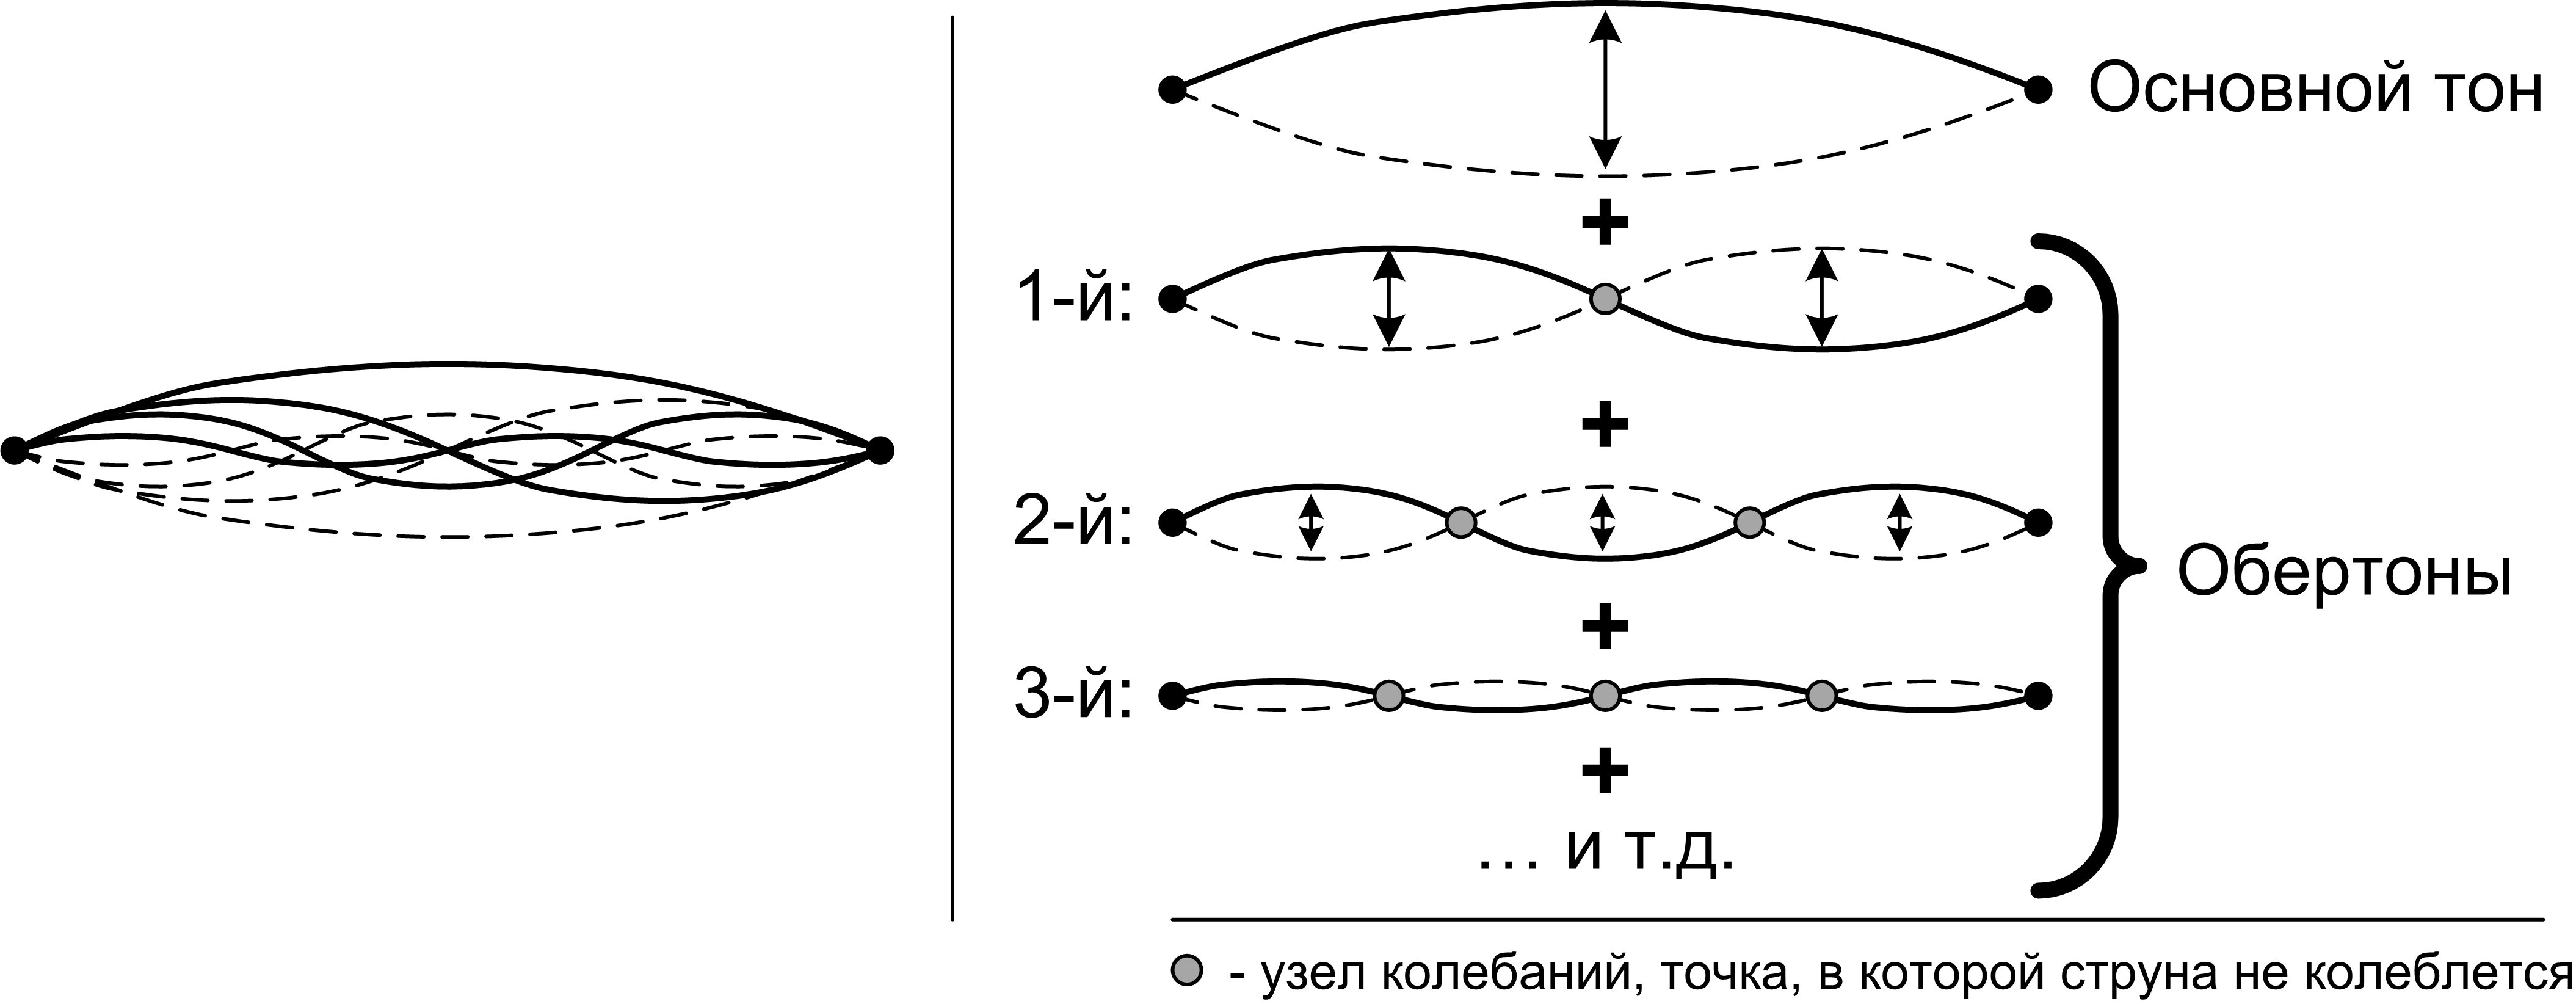
\includegraphics[width=0.95\textwidth]{figs/string-nodes}
    \end{center}
\end{frame}


\subsection{Порождаемый струной звук}

\begin{frame}
    \frametitle{Порождаемый струной звук}

    \begin{center}
        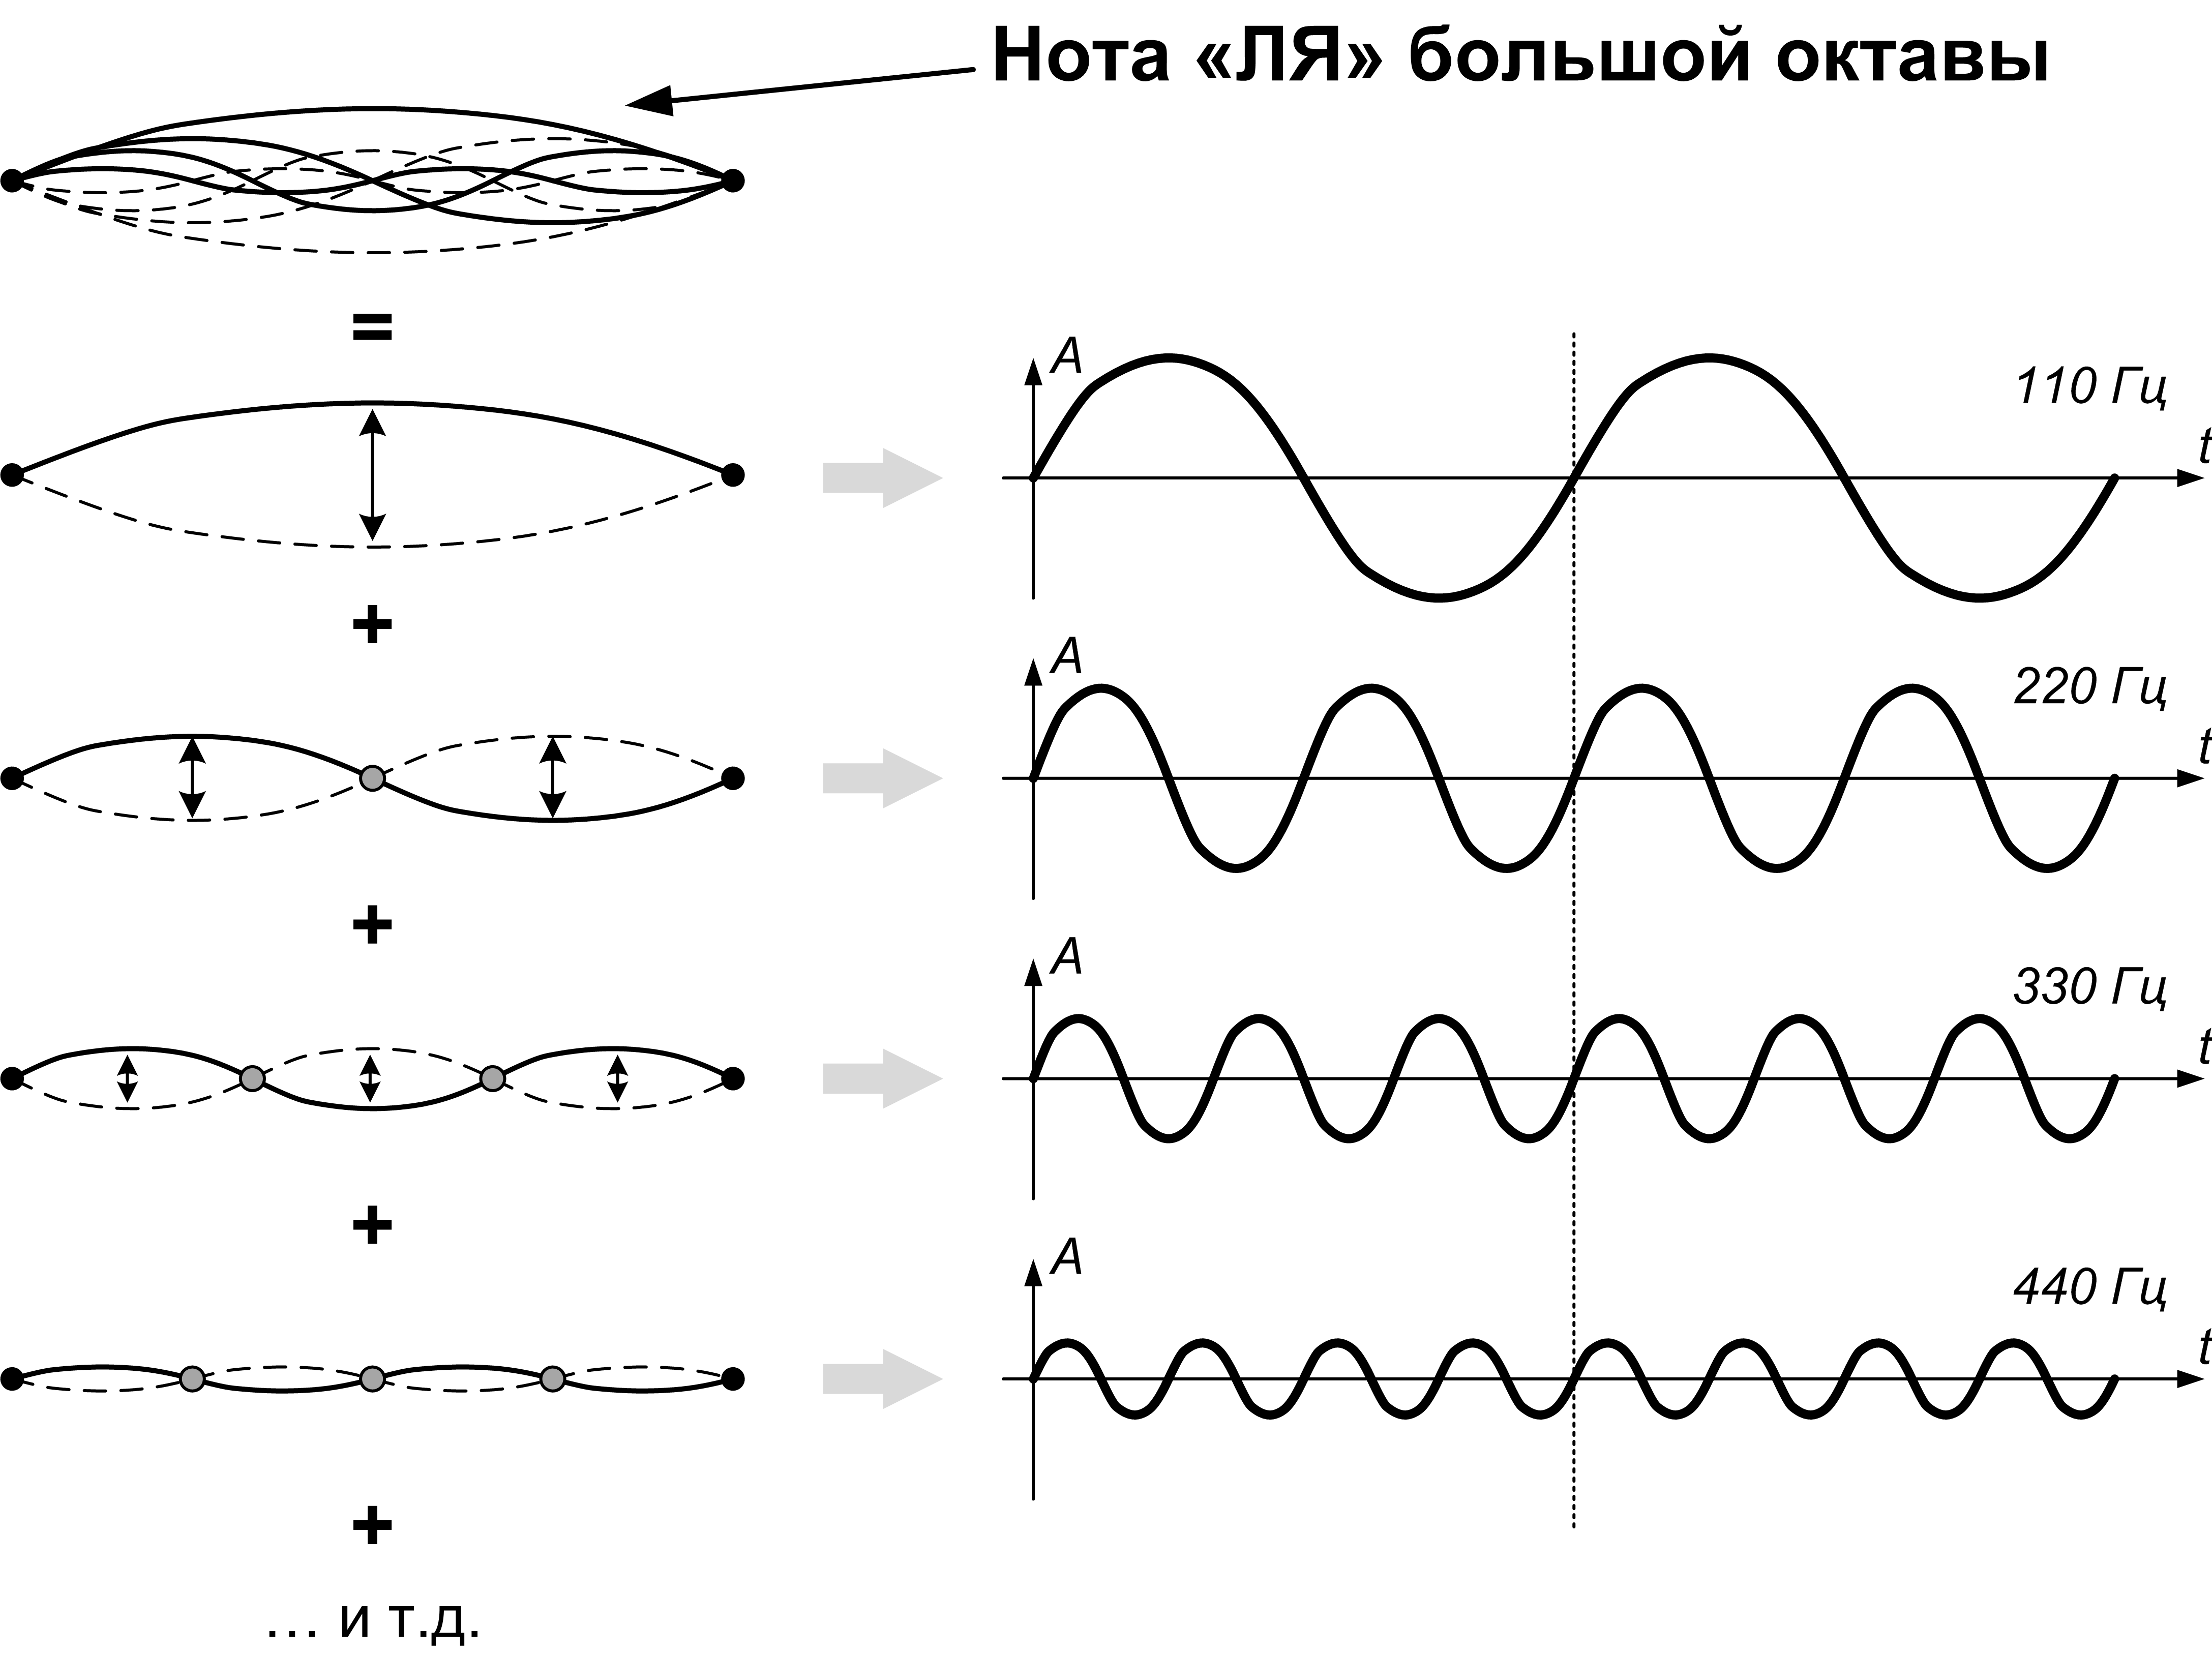
\includegraphics[width=0.8\textwidth]{figs/string-frequences}
    \end{center}
\end{frame}


\section{Цифровой сигнал VS аналоговый}


\subsection{Аналоговый сигнал}

\begin{frame}
    \frametitle{Аналоговый сигнал}

    \begin{center}
        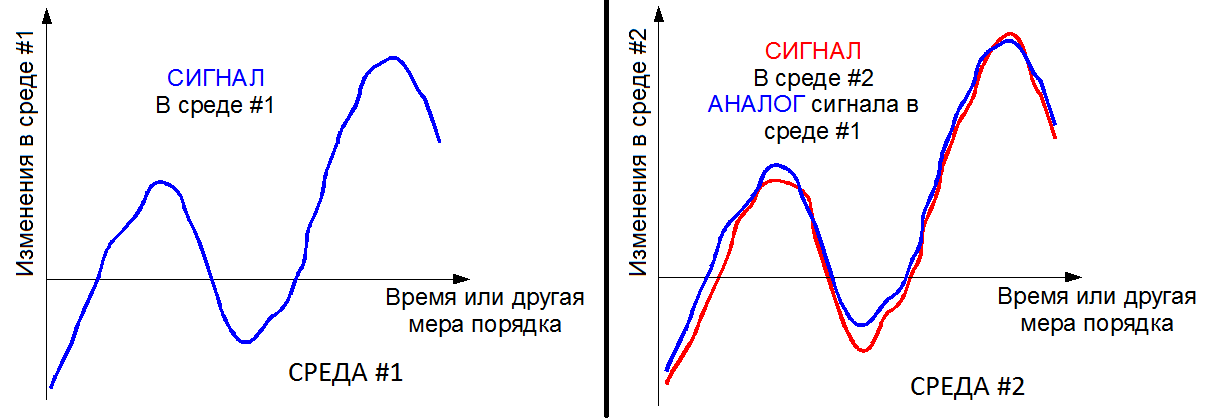
\includegraphics[width=\textwidth]{figs/analog}
    \end{center}
\end{frame}


\subsection{Цифровой сигнал}

\begin{frame}
    \frametitle{Цифровой сигнал}

    \begin{center}
        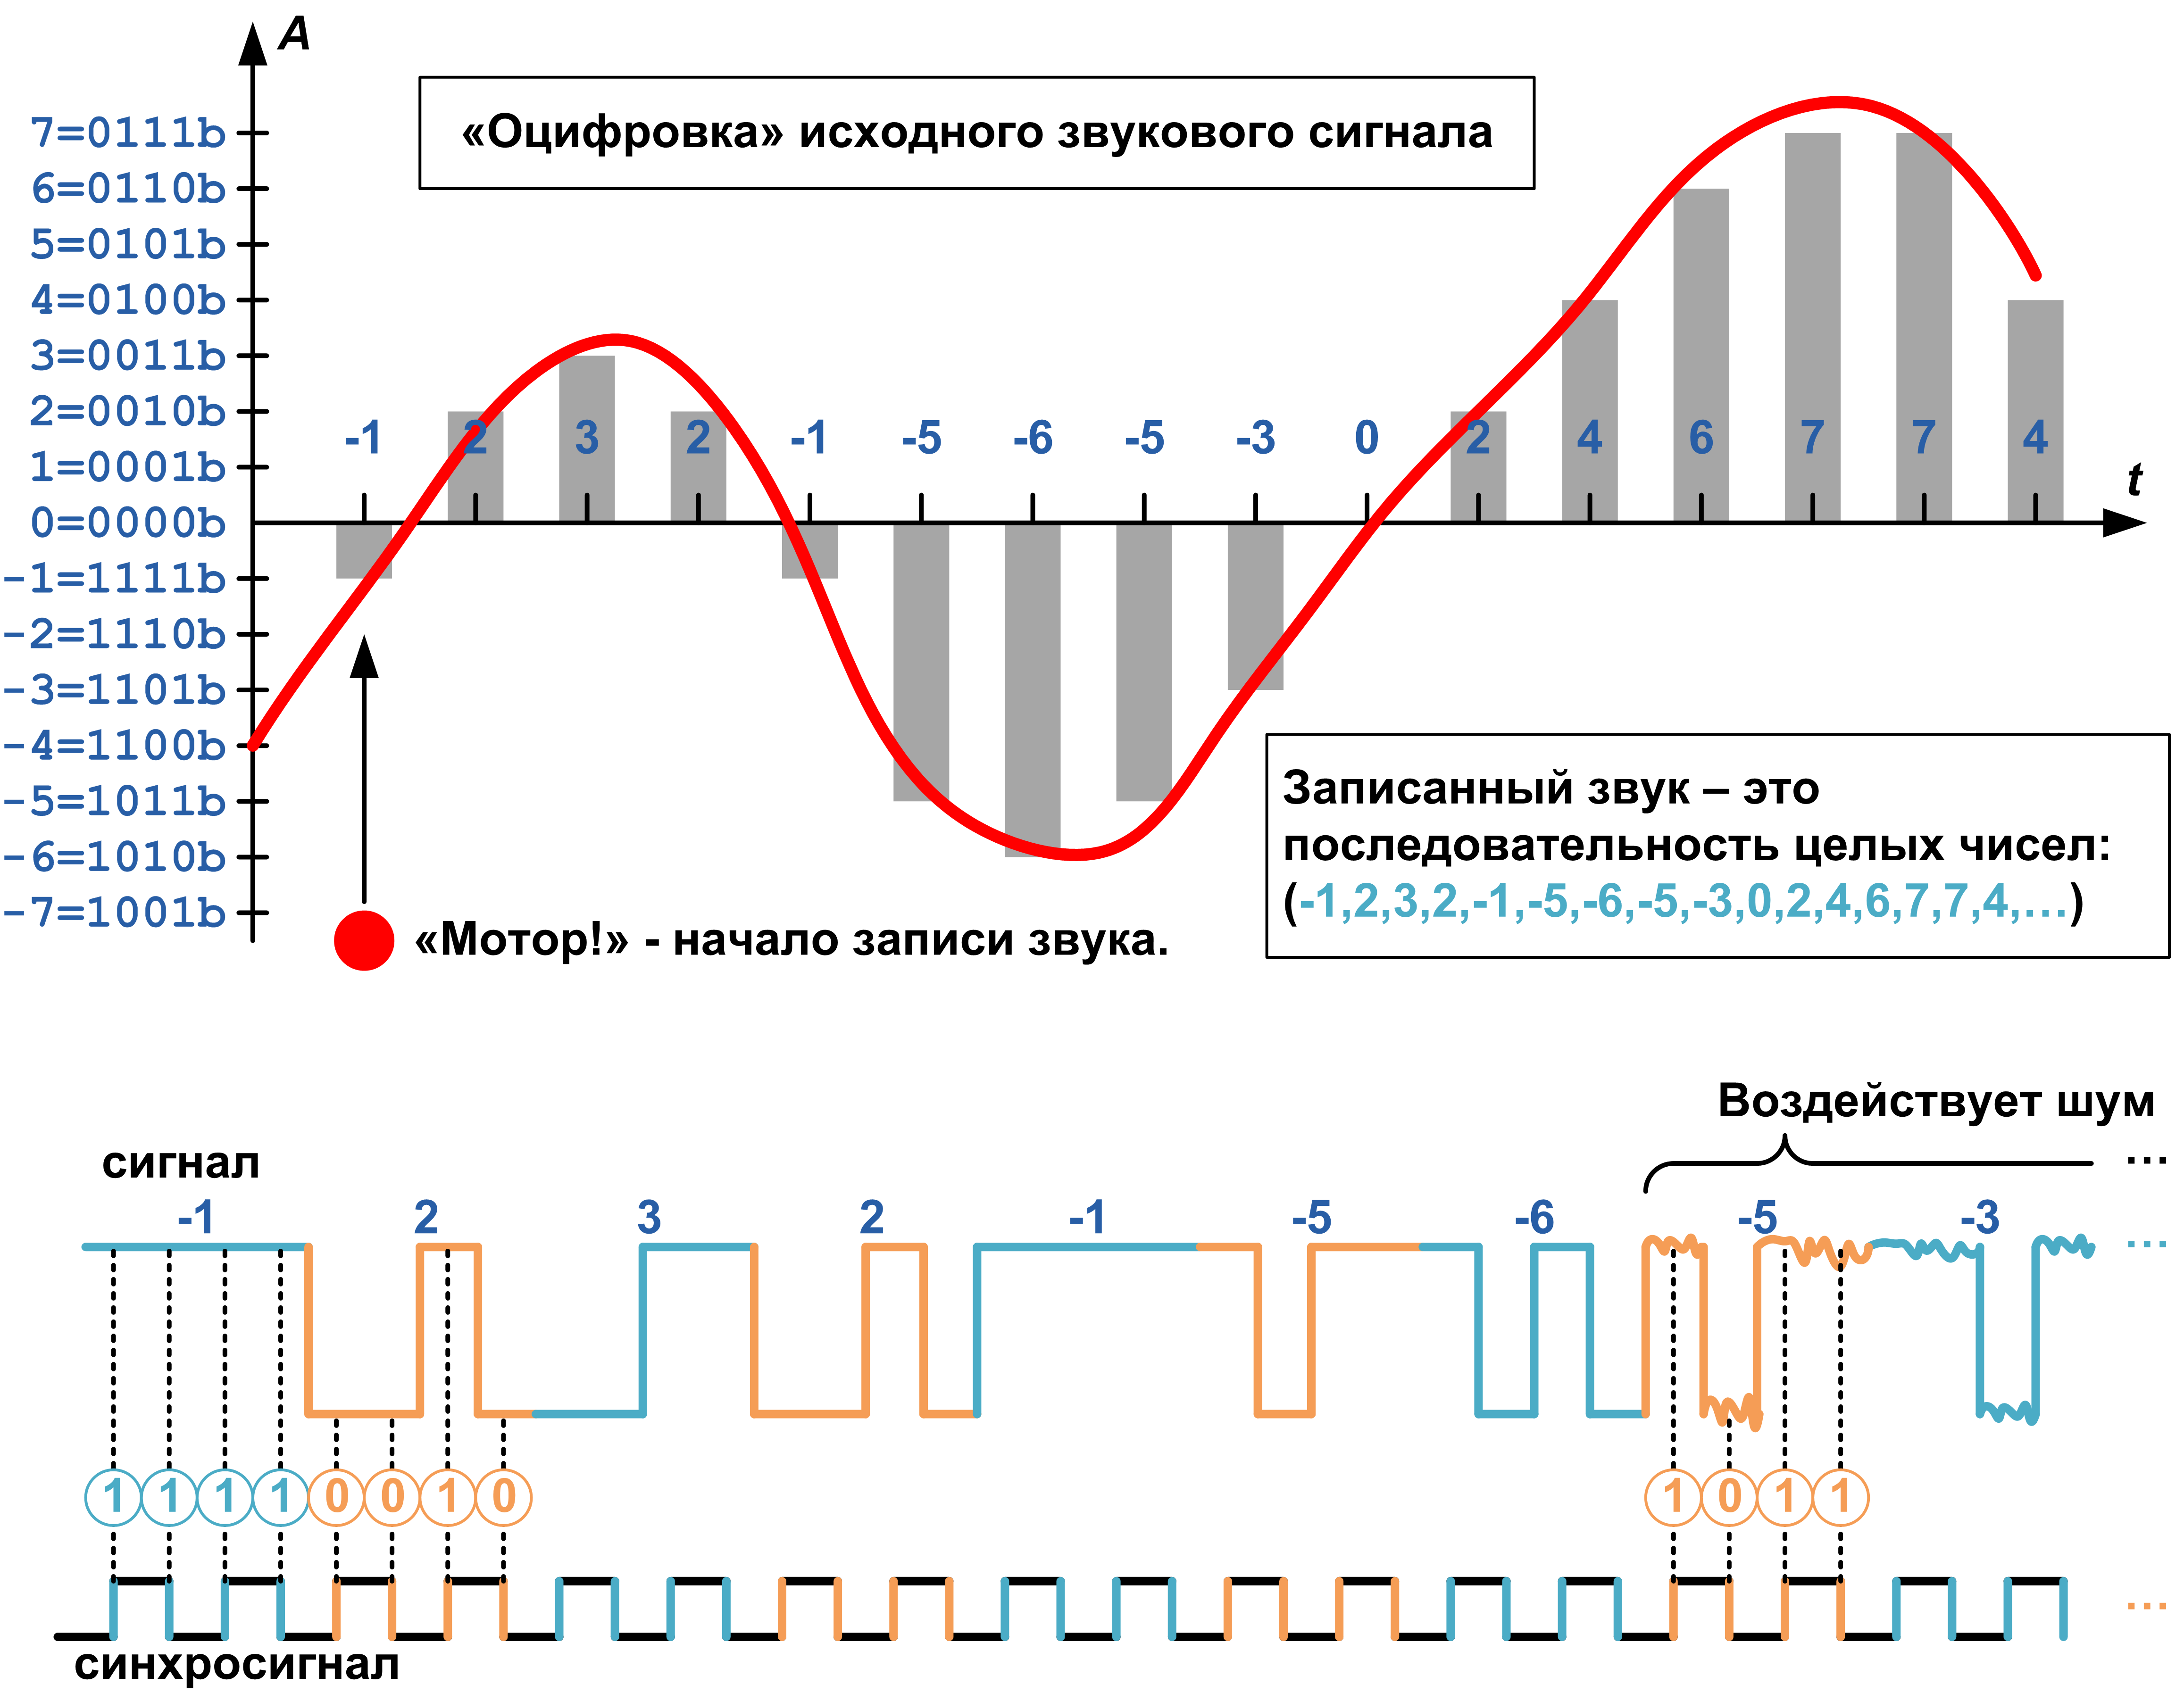
\includegraphics[width=0.8\textwidth]{figs/digital}
    \end{center}
\end{frame}


\section{Спектральный анализ флажолета}


\subsection{Фильтрация призвуков касанием пальца}


\begin{frame}
    \frametitle{Фильтрация призвуков касанием пальца}

    \begin{center}
        \only<1>{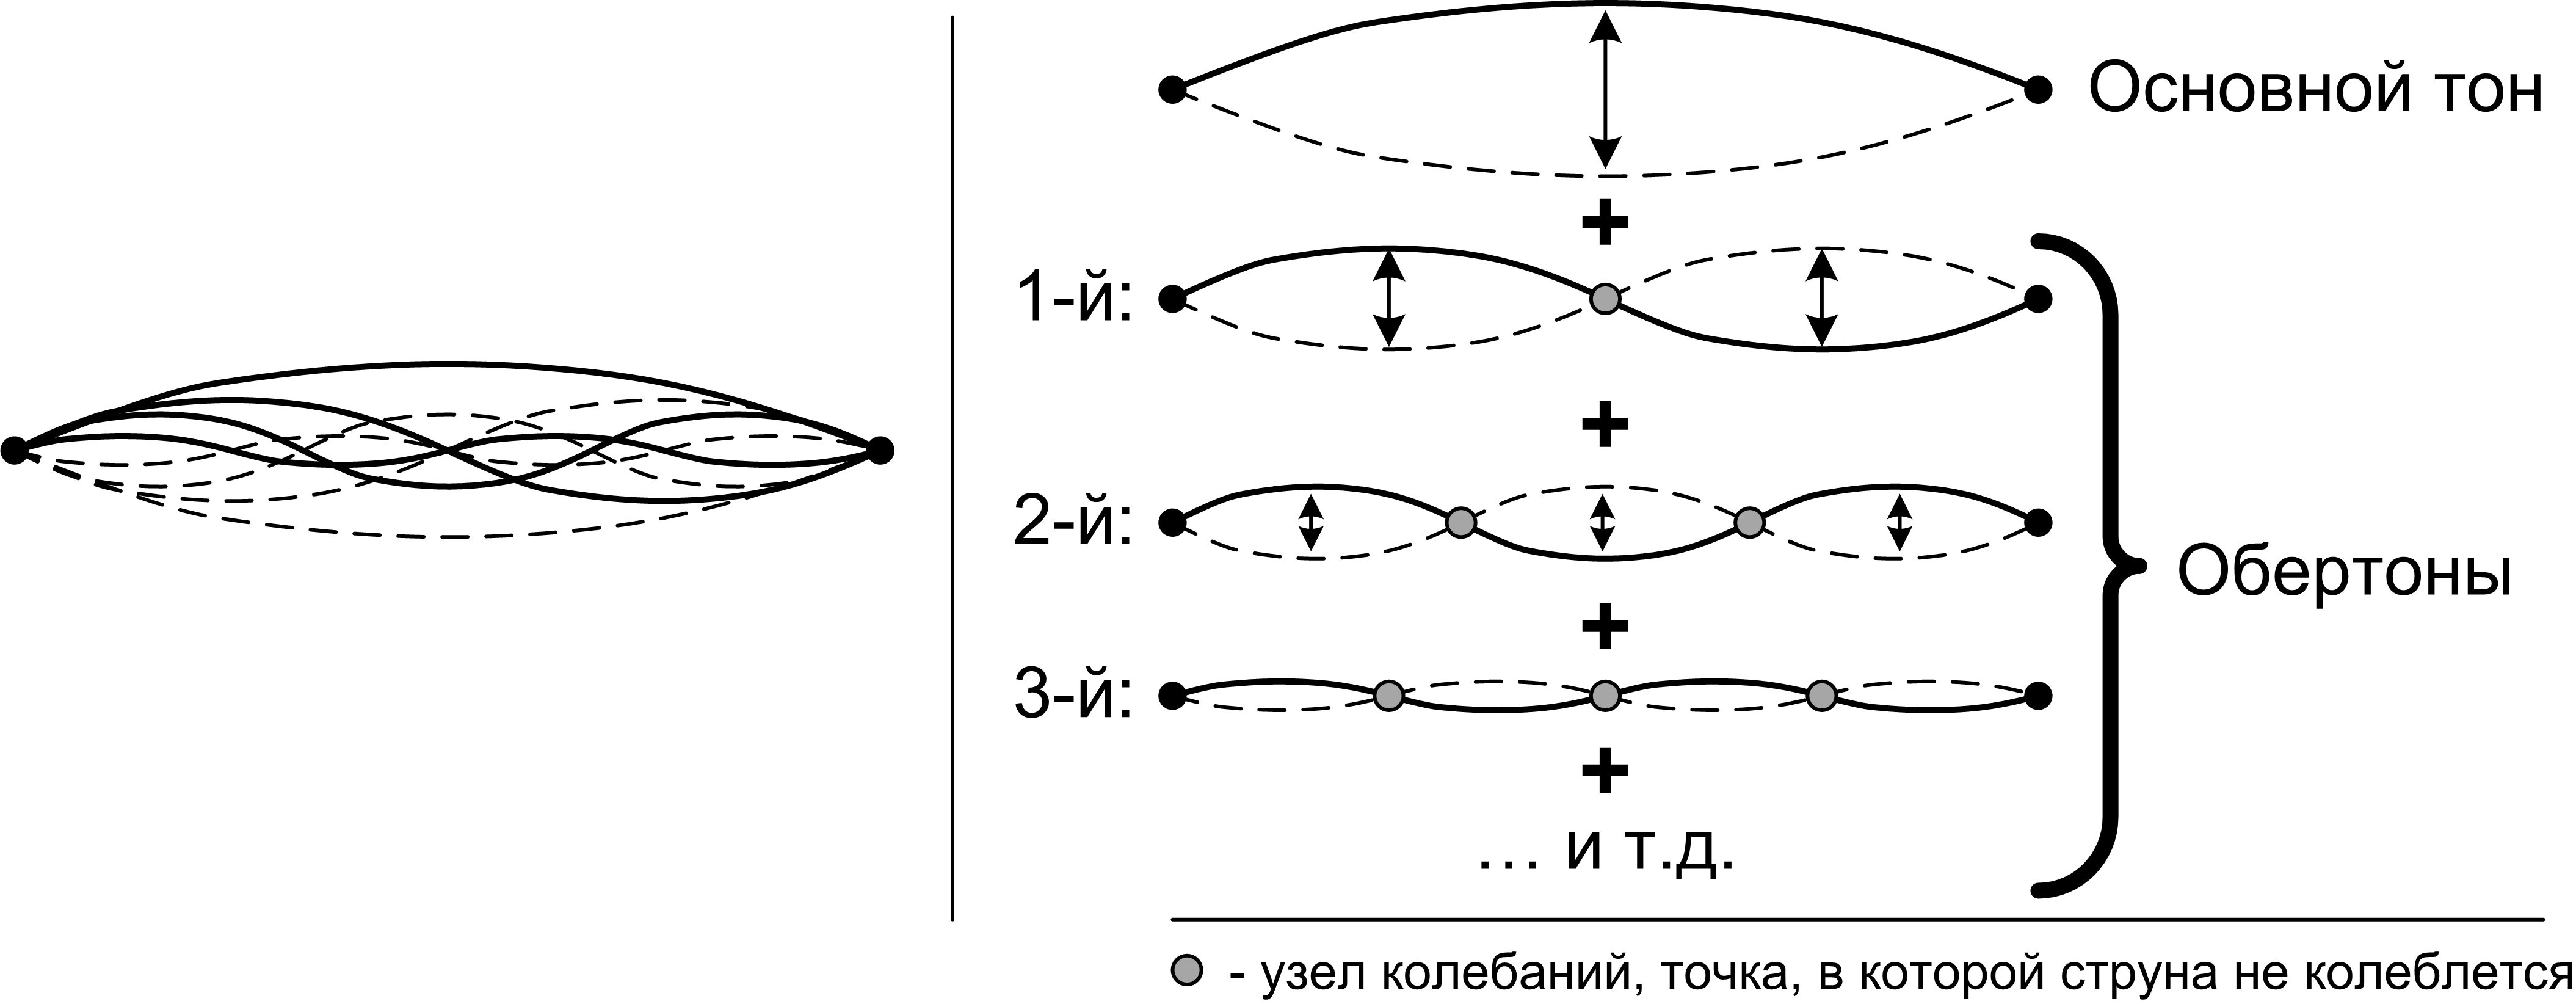
\includegraphics[width=\textwidth]{figs/string-nodes}}
        \only<2>{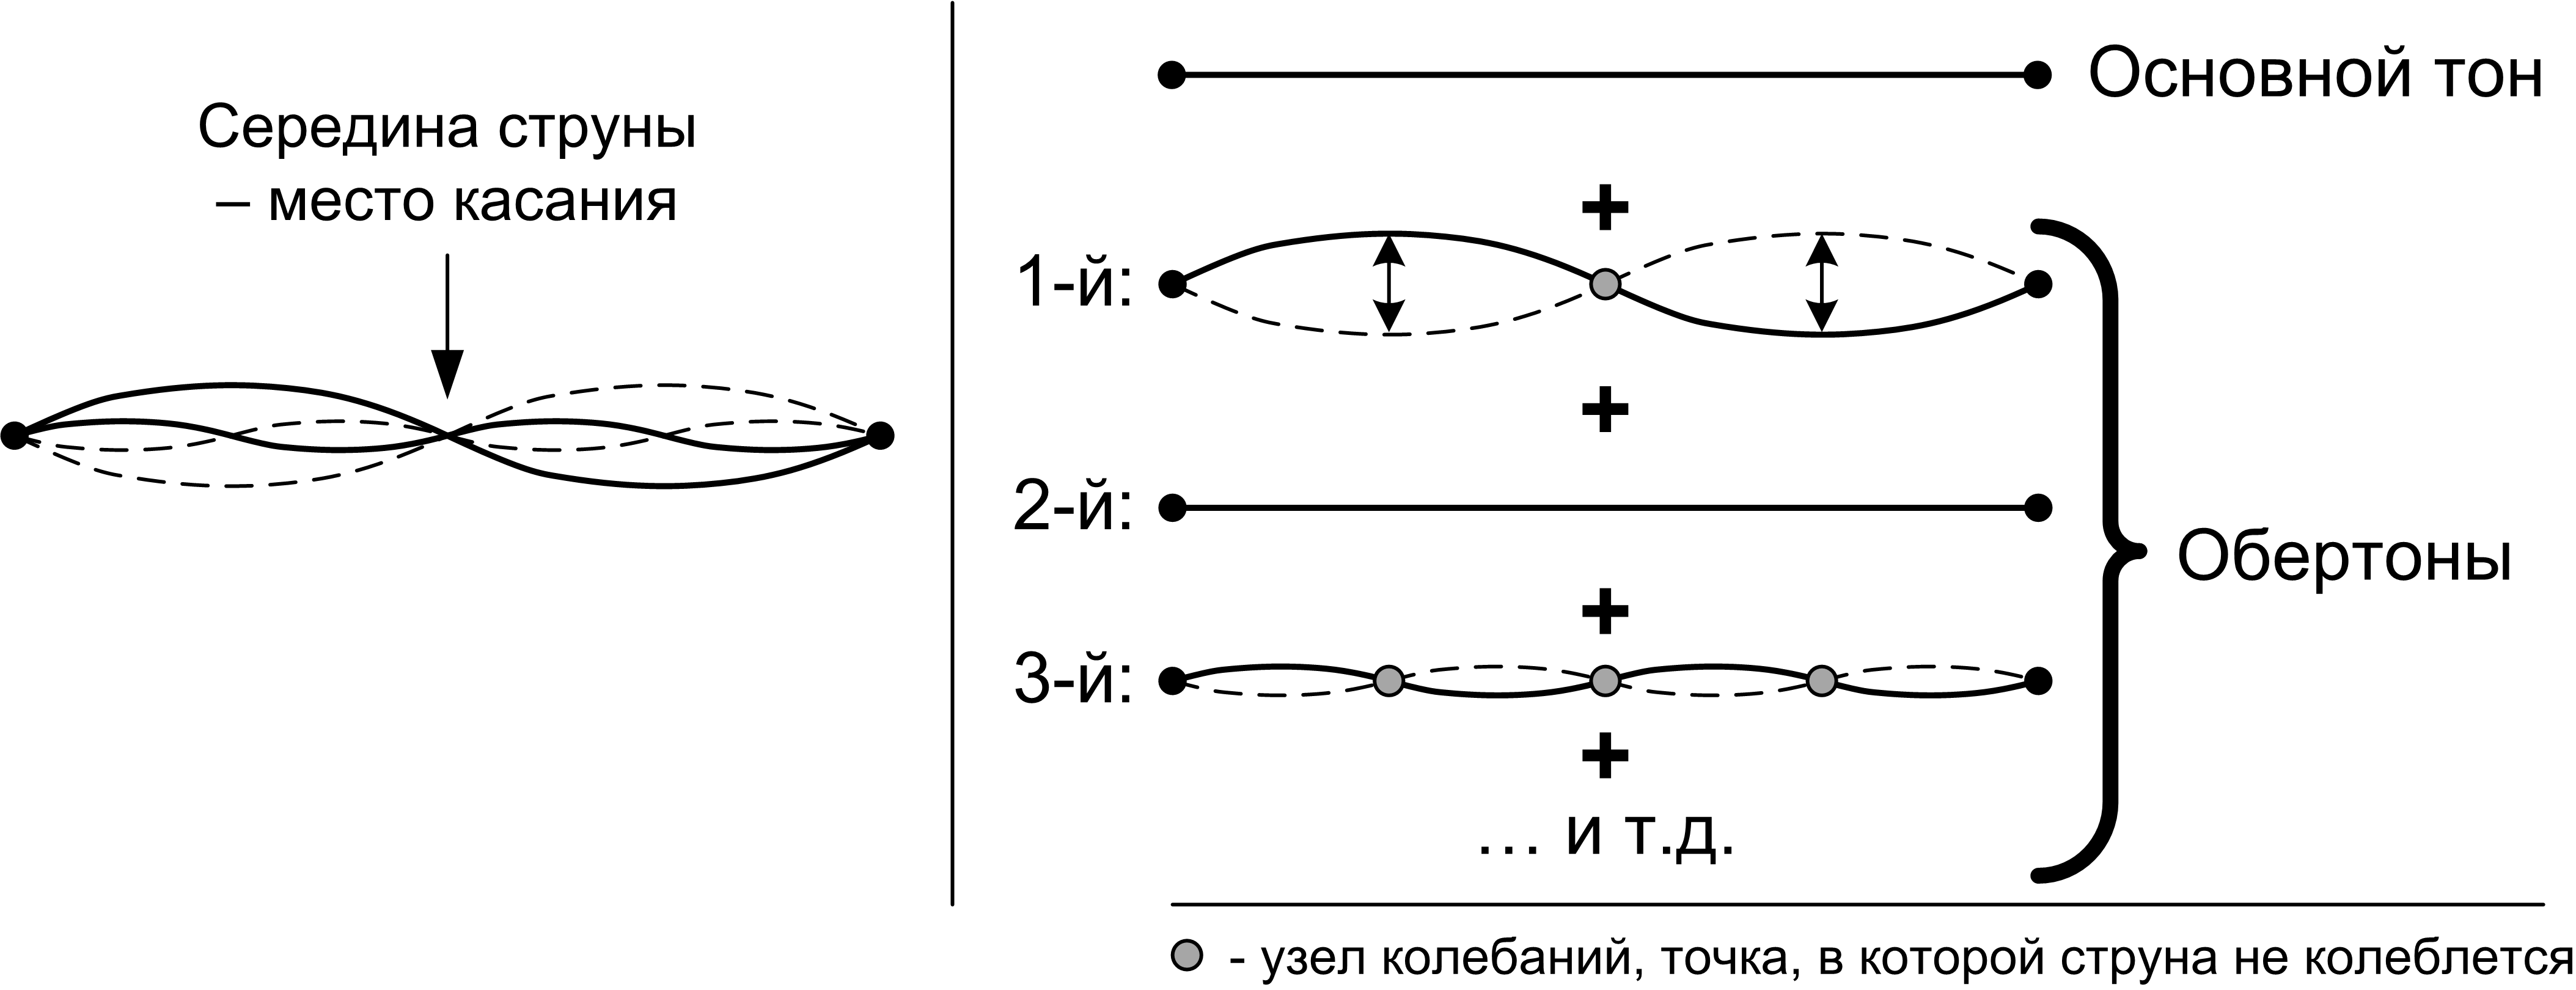
\includegraphics[width=\textwidth]{figs/string-flagolet}}
    \end{center}
\end{frame}


\subsection{А есть ли разница <<на слух>>?}

\begin{frame}
    \frametitle{А есть ли разница <<на слух>>?}

    \begin{center}
        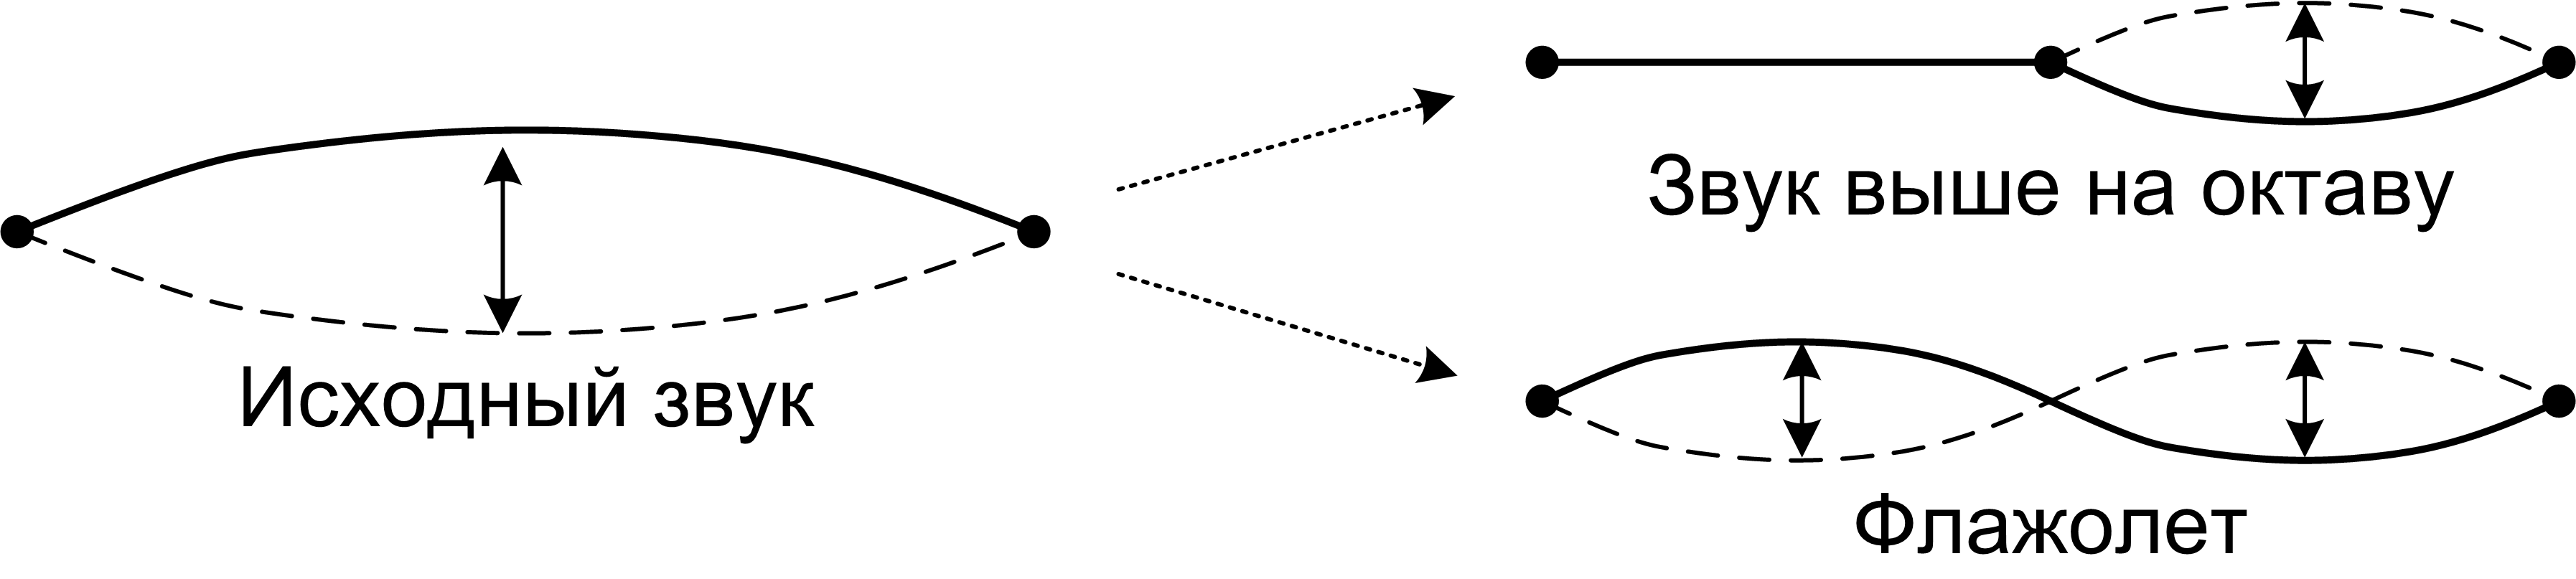
\includegraphics[width=\textwidth]{figs/string-flagol-vs-octave}
    \end{center}
\end{frame}


\appendix

\begin{frame}
    \frametitle{Окраска звука}

    \begin{center}
        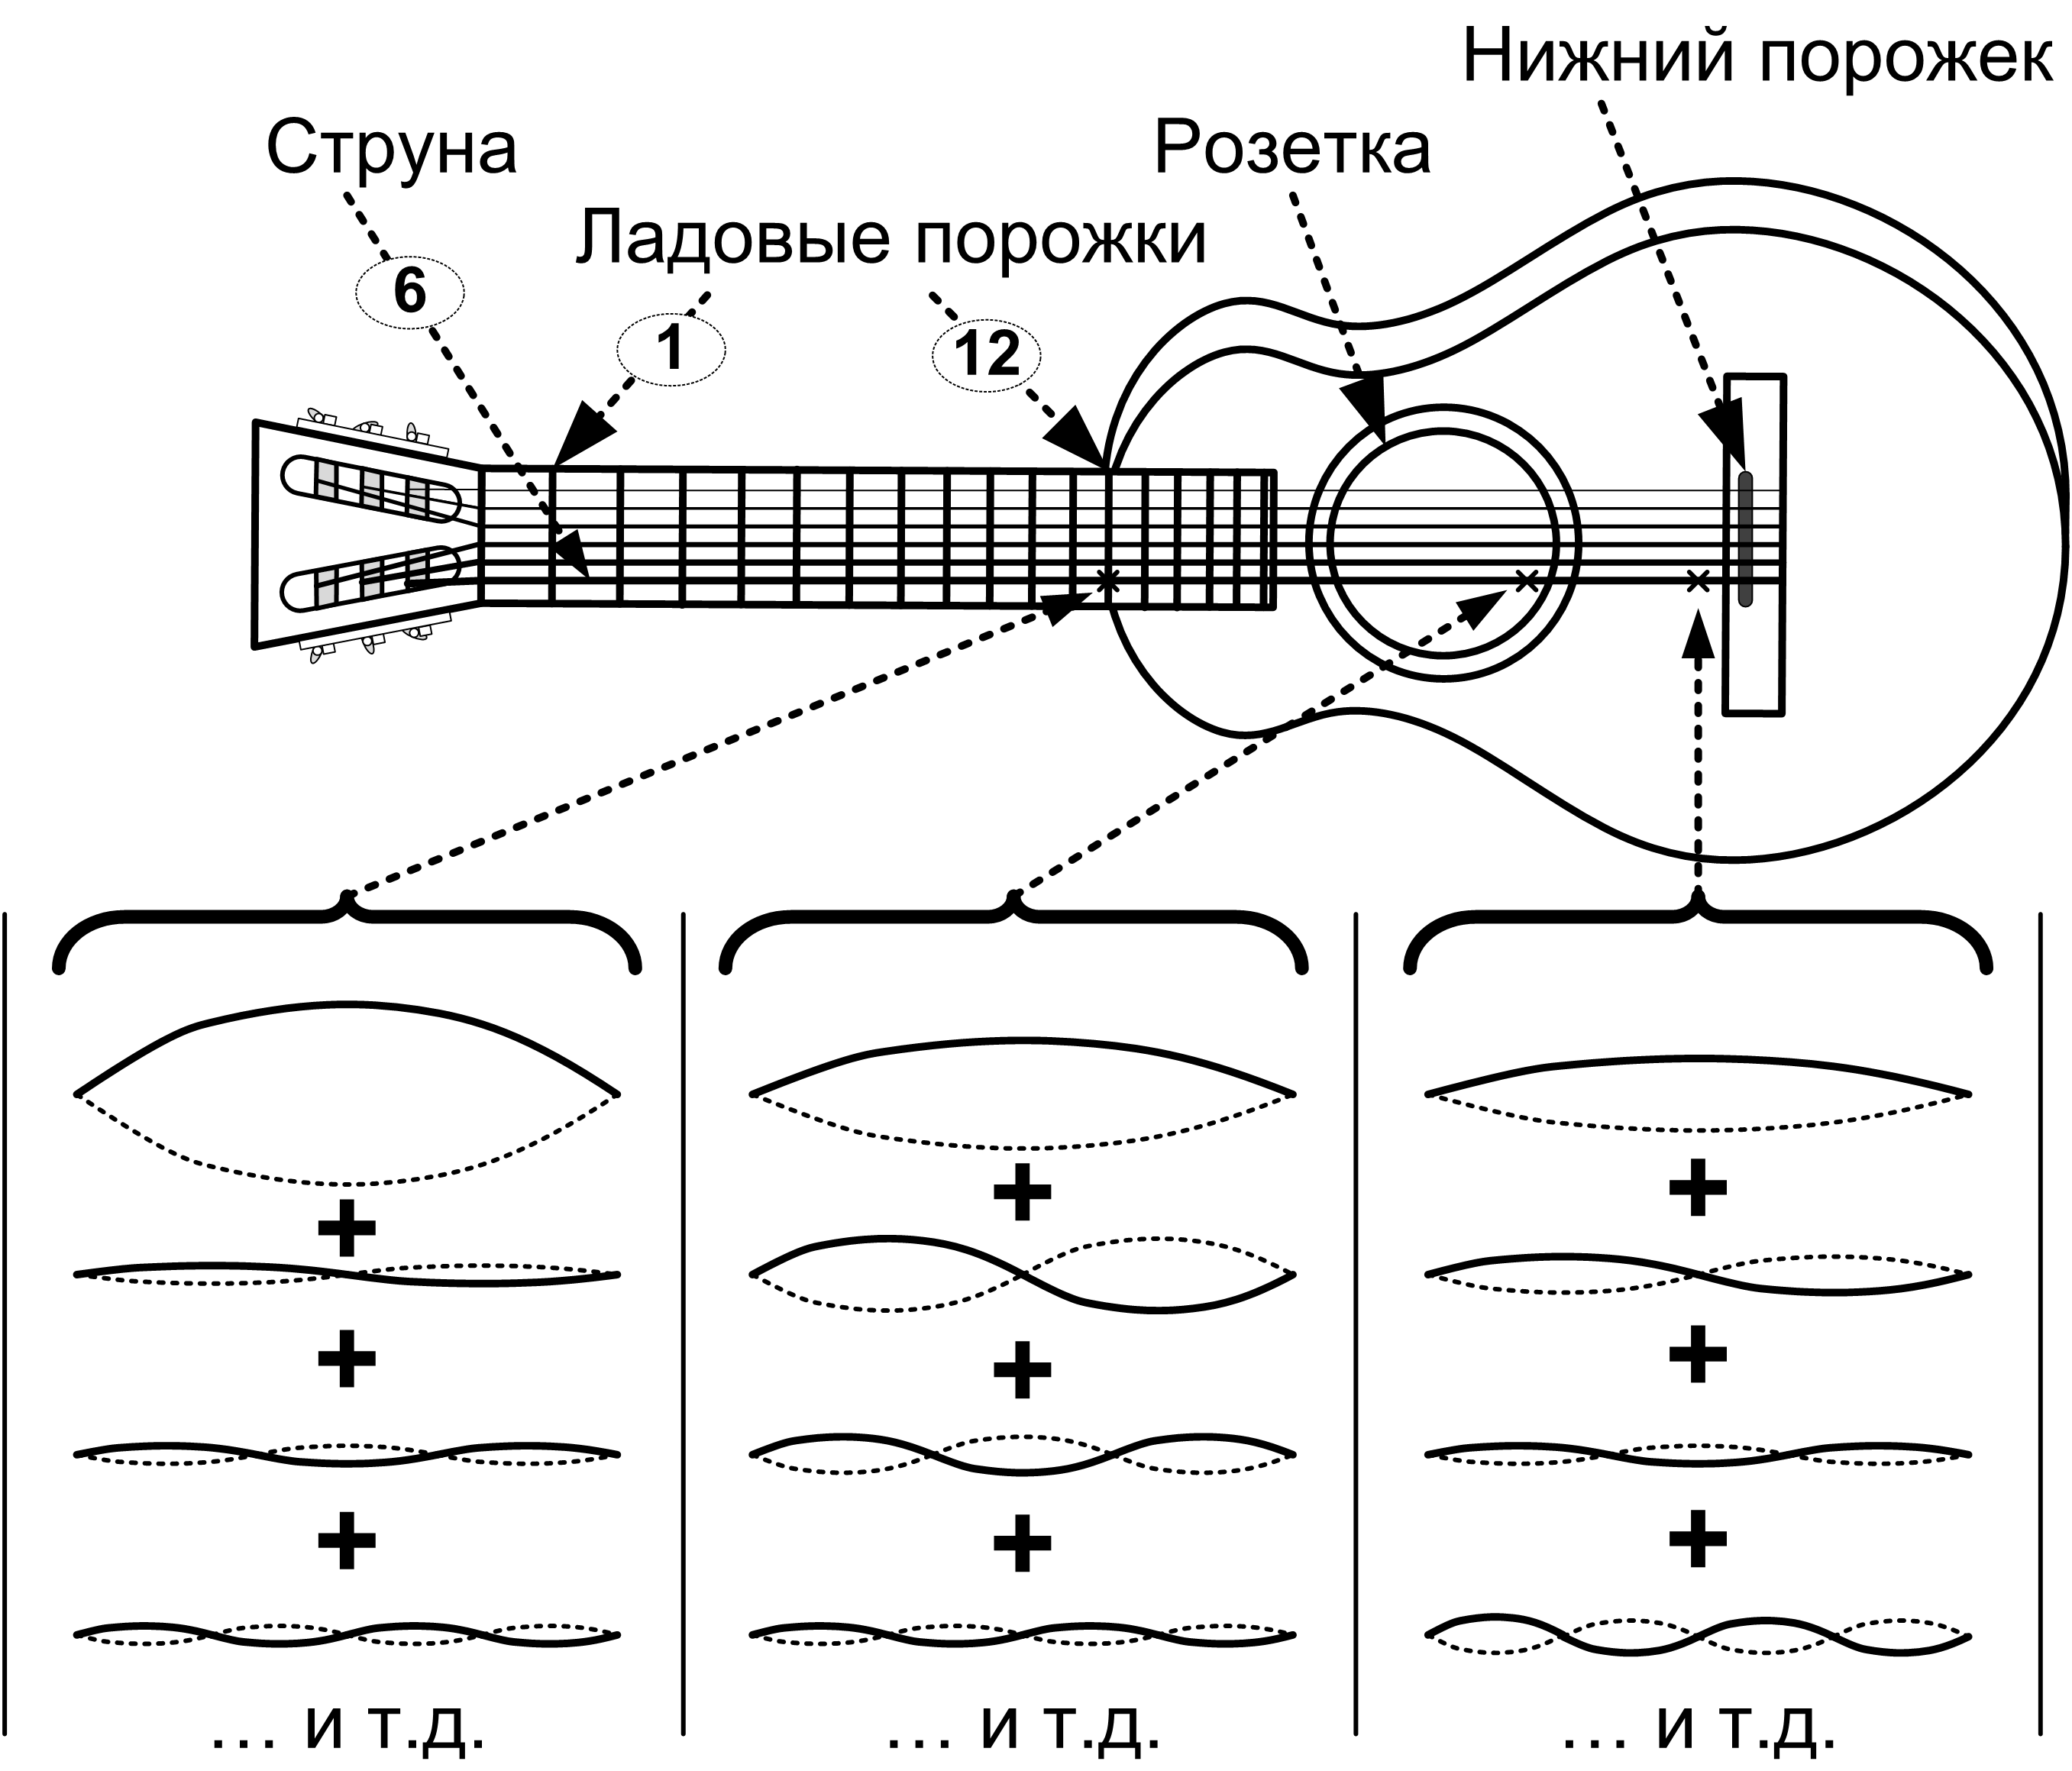
\includegraphics[width=.6\textwidth]{figs/obertone-color}
    \end{center}
\end{frame}

\end{document}